% Content-Aware Visual Chunking in Screenshot RAG: A Reader--Retriever Tradeoff
% Build: run  python paper/gen_paper_numbers.py  first (generates numbers.tex, tables/, figures/),
%        then compile with pdflatex/latexmk (e.g. on Overleaf). See paper/README.md.
% DATA DISCIPLINE: no number is hand-typed here; all come from % AUTO-GENERATED by paper/gen_paper_numbers.py — DO NOT EDIT. Every number sourced from results/*.json.

\newcommand{\BvBlockRatio}{5.0}
\newcommand{\BvCaBlock}{0.77}
\newcommand{\BvCaBlockN}{78}
\newcommand{\BvCaRow}{0.95}
\newcommand{\BvCaRowN}{68}
\newcommand{\BvFixedBlock}{3.82}
\newcommand{\BvFixedBlockN}{387}
\newcommand{\BvFixedRow}{5.42}
\newcommand{\BvFixedRowN}{387}
\newcommand{\BvRowRatio}{5.7}
\newcommand{\CaImgFlatDelta}{+0.12}
\newcommand{\CaImgHierDelta}{+0.28}
\newcommand{\CaTxtFlatDelta}{-0.08}
\newcommand{\CaTxtHierDelta}{+0.00}
\newcommand{\EmbedModel}{Qwen/Qwen3-VL-Embedding-2B}
\newcommand{\ImgCaSawGold}{96}
\newcommand{\ImgFixedSawGold}{100}
\newcommand{\InatCaFlatAcc}{0.56}
\newcommand{\InatCaHierAcc}{0.68}
\newcommand{\InatChunksCa}{417}
\newcommand{\InatChunksDeltaPct}{24.5}
\newcommand{\InatChunksFixed}{335}
\newcommand{\InatDistr}{15}
\newcommand{\InatFixedFlatAcc}{0.44}
\newcommand{\InatFixedHierAcc}{0.40}
\newcommand{\InatGold}{25}
\newcommand{\InatHStdCa}{329}
\newcommand{\InatHStdFixed}{82}
\newcommand{\InatImgRecallCa}{0.96}
\newcommand{\InatImgRecallFixed}{0.88}
\newcommand{\InatN}{25}
\newcommand{\InatPages}{40}
\newcommand{\InatReaderCeil}{8}
\newcommand{\InatRetrCeil}{0}
\newcommand{\InatTextCaFlatAcc}{0.36}
\newcommand{\InatTextCaHierAcc}{0.40}
\newcommand{\InatTextFixedFlatAcc}{0.44}
\newcommand{\InatTextFixedHierAcc}{0.40}
\newcommand{\InatTppCa}{10.43}
\newcommand{\InatTppFixed}{8.38}
\newcommand{\InatTxtRecallCa}{0.44}
\newcommand{\InatTxtRecallFixed}{0.48}
\newcommand{\JudgeModel}{gpt-4.1-2025-04-14}
\newcommand{\McNemarBaselineAcc}{0.44}
\newcommand{\McNemarBestAcc}{0.68}
\newcommand{\McNemarDelta}{+0.24}
\newcommand{\McNemarDiscordant}{6}
\newcommand{\McNemarFavor}{6}
\newcommand{\McNemarN}{25}
\newcommand{\McNemarP}{0.031}
\newcommand{\NqCaFlatAcc}{0.61}
\newcommand{\NqCaHierAcc}{0.61}
\newcommand{\NqChunksCa}{1680}
\newcommand{\NqChunksDeltaPct}{0.0}
\newcommand{\NqChunksFixed}{1680}
\newcommand{\NqDistr}{60}
\newcommand{\NqFixedFlatAcc}{0.64}
\newcommand{\NqFixedHierAcc}{0.59}
\newcommand{\NqGold}{150}
\newcommand{\NqHStdCa}{2}
\newcommand{\NqHStdFixed}{2}
\newcommand{\NqN}{150}
\newcommand{\NqPages}{210}
\newcommand{\NqReaderCeil}{46}
\newcommand{\NqRetrCeil}{12}
\newcommand{\NqTppCa}{8.00}
\newcommand{\NqTppFixed}{8.00}
\newcommand{\NqTxtRecallCa}{0.88}
\newcommand{\NqTxtRecallFixed}{0.88}
\newcommand{\NqtCaFlatAcc}{0.49}
\newcommand{\NqtCaHierAcc}{0.52}
\newcommand{\NqtChunksCa}{1680}
\newcommand{\NqtChunksDeltaPct}{0.0}
\newcommand{\NqtChunksFixed}{1680}
\newcommand{\NqtDistr}{60}
\newcommand{\NqtFixedFlatAcc}{0.49}
\newcommand{\NqtFixedHierAcc}{0.54}
\newcommand{\NqtGold}{150}
\newcommand{\NqtHStdCa}{2}
\newcommand{\NqtHStdFixed}{2}
\newcommand{\NqtN}{150}
\newcommand{\NqtPages}{210}
\newcommand{\NqtReaderCeil}{56}
\newcommand{\NqtRetrCeil}{16}
\newcommand{\NqtTppCa}{8.00}
\newcommand{\NqtTppFixed}{8.00}
\newcommand{\NqtTxtRecallCa}{0.85}
\newcommand{\NqtTxtRecallFixed}{0.85}
\newcommand{\ReaderCeilPctMax}{100}
\newcommand{\ReaderCeilPctMin}{78}
\newcommand{\ReaderModel}{gpt-4o}
\newcommand{\TxtCaSawGold}{56}
\newcommand{\TxtFixedSawGold}{68}
 or tables/.
\documentclass[11pt]{article}

\usepackage[utf8]{inputenc}
\usepackage[T1]{fontenc}
\usepackage[margin=1in]{geometry}
\usepackage{microtype}
\usepackage{amsmath,amssymb}
\usepackage{graphicx}
\usepackage{booktabs}
\usepackage{caption}
\usepackage{authblk}
\usepackage[numbers,sort&compress]{natbib}
\usepackage[hidelinks]{hyperref}

\graphicspath{{figures/}}
% AUTO-GENERATED by paper/gen_paper_numbers.py — DO NOT EDIT. Every number sourced from results/*.json.

\newcommand{\BvBlockRatio}{5.0}
\newcommand{\BvCaBlock}{0.77}
\newcommand{\BvCaBlockN}{78}
\newcommand{\BvCaRow}{0.95}
\newcommand{\BvCaRowN}{68}
\newcommand{\BvFixedBlock}{3.82}
\newcommand{\BvFixedBlockN}{387}
\newcommand{\BvFixedRow}{5.42}
\newcommand{\BvFixedRowN}{387}
\newcommand{\BvRowRatio}{5.7}
\newcommand{\CaImgFlatDelta}{+0.12}
\newcommand{\CaImgHierDelta}{+0.28}
\newcommand{\CaTxtFlatDelta}{-0.08}
\newcommand{\CaTxtHierDelta}{+0.00}
\newcommand{\EmbedModel}{Qwen/Qwen3-VL-Embedding-2B}
\newcommand{\ImgCaSawGold}{96}
\newcommand{\ImgFixedSawGold}{100}
\newcommand{\InatCaFlatAcc}{0.56}
\newcommand{\InatCaHierAcc}{0.68}
\newcommand{\InatChunksCa}{417}
\newcommand{\InatChunksDeltaPct}{24.5}
\newcommand{\InatChunksFixed}{335}
\newcommand{\InatDistr}{15}
\newcommand{\InatFixedFlatAcc}{0.44}
\newcommand{\InatFixedHierAcc}{0.40}
\newcommand{\InatGold}{25}
\newcommand{\InatHStdCa}{329}
\newcommand{\InatHStdFixed}{82}
\newcommand{\InatImgRecallCa}{0.96}
\newcommand{\InatImgRecallFixed}{0.88}
\newcommand{\InatN}{25}
\newcommand{\InatPages}{40}
\newcommand{\InatReaderCeil}{8}
\newcommand{\InatRetrCeil}{0}
\newcommand{\InatTextCaFlatAcc}{0.36}
\newcommand{\InatTextCaHierAcc}{0.40}
\newcommand{\InatTextFixedFlatAcc}{0.44}
\newcommand{\InatTextFixedHierAcc}{0.40}
\newcommand{\InatTppCa}{10.43}
\newcommand{\InatTppFixed}{8.38}
\newcommand{\InatTxtRecallCa}{0.44}
\newcommand{\InatTxtRecallFixed}{0.48}
\newcommand{\JudgeModel}{gpt-4.1-2025-04-14}
\newcommand{\McNemarBaselineAcc}{0.44}
\newcommand{\McNemarBestAcc}{0.68}
\newcommand{\McNemarDelta}{+0.24}
\newcommand{\McNemarDiscordant}{6}
\newcommand{\McNemarFavor}{6}
\newcommand{\McNemarN}{25}
\newcommand{\McNemarP}{0.031}
\newcommand{\NqCaFlatAcc}{0.61}
\newcommand{\NqCaHierAcc}{0.61}
\newcommand{\NqChunksCa}{1680}
\newcommand{\NqChunksDeltaPct}{0.0}
\newcommand{\NqChunksFixed}{1680}
\newcommand{\NqDistr}{60}
\newcommand{\NqFixedFlatAcc}{0.64}
\newcommand{\NqFixedHierAcc}{0.59}
\newcommand{\NqGold}{150}
\newcommand{\NqHStdCa}{2}
\newcommand{\NqHStdFixed}{2}
\newcommand{\NqN}{150}
\newcommand{\NqPages}{210}
\newcommand{\NqReaderCeil}{46}
\newcommand{\NqRetrCeil}{12}
\newcommand{\NqTppCa}{8.00}
\newcommand{\NqTppFixed}{8.00}
\newcommand{\NqTxtRecallCa}{0.88}
\newcommand{\NqTxtRecallFixed}{0.88}
\newcommand{\NqtCaFlatAcc}{0.49}
\newcommand{\NqtCaHierAcc}{0.52}
\newcommand{\NqtChunksCa}{1680}
\newcommand{\NqtChunksDeltaPct}{0.0}
\newcommand{\NqtChunksFixed}{1680}
\newcommand{\NqtDistr}{60}
\newcommand{\NqtFixedFlatAcc}{0.49}
\newcommand{\NqtFixedHierAcc}{0.54}
\newcommand{\NqtGold}{150}
\newcommand{\NqtHStdCa}{2}
\newcommand{\NqtHStdFixed}{2}
\newcommand{\NqtN}{150}
\newcommand{\NqtPages}{210}
\newcommand{\NqtReaderCeil}{56}
\newcommand{\NqtRetrCeil}{16}
\newcommand{\NqtTppCa}{8.00}
\newcommand{\NqtTppFixed}{8.00}
\newcommand{\NqtTxtRecallCa}{0.85}
\newcommand{\NqtTxtRecallFixed}{0.85}
\newcommand{\ReaderCeilPctMax}{100}
\newcommand{\ReaderCeilPctMin}{78}
\newcommand{\ReaderModel}{gpt-4o}
\newcommand{\TxtCaSawGold}{56}
\newcommand{\TxtFixedSawGold}{68}
     % auto-generated \newcommand macros (paper/gen_paper_numbers.py)
\setlength{\emergencystretch}{3em}  % absorb minor overfull \hbox warnings

\title{\bfseries Content-Aware Visual Chunking in Screenshot RAG:\\ A Reader--Retriever Tradeoff}
\author[1]{Kaushik Chaturvedula\thanks{Independent research. Correspondence: \texttt{kaushikchaturvedula@gmail.com}.}}
\affil[1]{\textit{Independent Researcher}}
\date{\today}

\begin{document}
\maketitle

\begin{abstract}
\noindent
Screenshot-based retrieval-augmented generation (\emph{pixel RAG}) renders documents to images and
answers questions over retrieved image tiles, sidestepping text extraction and preserving layout,
tables, and figures. A natural refinement is \textbf{content-aware chunking}: cutting tiles along
document structure rather than a fixed pixel grid, on the intuition that respecting content boundaries
should aid both retrieval and reading. Testing this on a screenshot-RAG pipeline across three document
types, we find a more nuanced picture than the intuition predicts. First, content-aware chunking is
\textbf{layout-gated}: on uniformly formatted Wikipedia prose and tables it produces tiles
\emph{byte-identical} to fixed-grid chunking (\NqtChunksFixed\ vs.\ \NqtChunksCa\ chunks) and has no
effect, engaging only on visually heterogeneous documents. Second, where it does change tiling, its QA
effect is governed by a \textbf{reader--retriever tradeoff}: finer, content-aligned tiles help the
vision--language reader extract answers but \emph{reduce} retrieval recall. Which effect dominates
depends on query modality. Under image queries, where retrieval is already saturated, content-aware
chunking raises QA accuracy by as much as \CaImgHierDelta\ absolute; \emph{but this gain is
regime-specific}: under text queries on the same corpus with identical tiles it vanishes or reverses
(\CaTxtFlatDelta\,/\,\CaTxtHierDelta), as smaller tiles lower gold-page retrieval from
\TxtFixedSawGold\%\ to \TxtCaSawGold\%. Third, across all settings \ReaderCeilPctMin--\ReaderCeilPctMax\%\
of QA errors occur on \emph{correctly-retrieved} content, indicating the reader---not chunking or
retrieval---is the dominant bottleneck. We therefore caution against treating content-aware visual
chunking as a general improvement, and instead characterize precisely when it helps and when it hurts.
\end{abstract}

\section{Introduction}\label{sec:intro}
Retrieval-augmented generation (RAG) over documents conventionally extracts text, chunks it, embeds the
chunks, and feeds retrieved passages to a language model. \textbf{Screenshot-based (pixel) RAG} takes a
different path: it renders each document page to an image, splits the image into tiles, embeds the tiles
with a vision encoder, retrieves tiles for a query, and answers with a vision--language model (VLM)
reading the \emph{pixels}---never extracting text~\citep{pixelrag}. This sidesteps brittle parsing and
natively preserves tables, figures, math, and layout that text extraction destroys.

Pixel RAG inherits one design choice directly from text RAG: \emph{how to chunk}. The default is a
fixed pixel grid---slice each page into equal-height tiles. This is structurally blind: a tile boundary
can fall in the middle of a table row, a paragraph, or a figure. A natural refinement, mirroring
semantic chunking in text RAG, is \textbf{content-aware chunking}: place tile boundaries along document
structure (block and table-row boundaries) so that no coherent region is split~\citep{m3docdep,colchunk}.
The intuition is twofold---content-aligned tiles should retrieve better (a query matches a self-contained
unit) and read better (the VLM sees an intact region)---and it is tempting to adopt as a general
improvement.

\textbf{We test that intuition} with a controlled $2\times2$ ablation---chunker $\{$fixed,
content-aware$\}$ $\times$ retrieval $\{$flat, hierarchical-expand$\}$---on a screenshot-RAG pipeline
across three document types spanning image- and text-primary queries. The answer is \emph{conditional,
not a general yes}, and the conditions are themselves the finding: (i) content-aware chunking is a
\emph{no-op} on uniformly formatted documents, where it emits tiles byte-identical to the fixed grid, so
it can only act on visually heterogeneous layouts; (ii) where it does act, finer content-aligned tiles
trade \emph{better reading} against \emph{worse retrieval}, and \textbf{query modality} decides which
effect wins; and (iii) regardless of chunking, most QA failures are the \emph{reader} misreading content
it was correctly given, not retrieval missing it. We \textbf{do not claim content-aware visual chunking
improves QA}---the data refutes that as a general statement. Our contribution is the characterization of
when it helps and hurts, and the reader--retriever mechanism behind it.

\paragraph{Contributions.}
\begin{enumerate}\setlength\itemsep{1pt}
  \item A controlled $2\times2$ (chunker $\times$ retrieval) ablation of content-aware vs.\ fixed-grid
        visual chunking on a screenshot-RAG pipeline across three document types.
  \item A \textbf{layout-gating} finding: content-aware chunking is a no-op on uniform layouts, producing
        byte-identical tiles (\NqtChunksFixed\ vs.\ \NqtChunksCa\ chunks on both text corpora)---a
        methodological caution for the visual-chunking literature, where uniform-layout benchmarks cannot
        test the method.
  \item A \textbf{same-corpus, same-tiles modality-flip} experiment isolating the chunking benefit as
        image-query-specific (content-aware effect \CaImgFlatDelta\,/\,\CaImgHierDelta\ under image queries
        vs.\ \CaTxtFlatDelta\,/\,\CaTxtHierDelta\ under text queries), revealing the reader--retriever tradeoff.
  \item A \textbf{reader-ceiling diagnostic} showing \ReaderCeilPctMin--\ReaderCeilPctMax\%\ of failures are
        reading errors on correctly-retrieved content, redirecting effort toward reader capacity rather
        than chunking or retrieval sophistication.
\end{enumerate}

\section{Related Work}\label{sec:related}
\paragraph{Screenshot / pixel RAG.} Rather than parsing documents to text, pixel-native retrieval renders
pages and retrieves over image tiles, reading answers directly from pixels~\citep{pixelrag}. This
preserves tables, figures, and layout that text extraction discards, at the cost of importing image-space
design choices such as tiling. This line descends from late-interaction visual document retrieval, which
embeds page images directly rather than extracted text~\citep{colpali}.

\paragraph{Visual document chunking.} Several recent systems cut visual documents along structure rather
than a fixed grid: region- and dependency-aware document chunking~\citep{m3docdep}, visual late chunking
that aligns embeddings to content units~\citep{colchunk}, and hierarchical multimodal retrieval over
structured documents~\citep{mhierrag}. These works motivate content-aware visual chunking; we instead
\emph{characterize} when it helps and hurts, and report a layout-gating no-op that uniform-layout
benchmarks would miss.

\paragraph{Hierarchical / tree-structured RAG.} Tree-organized retrieval summarizes and indexes documents
at multiple granularities~\citep{raptor}; reasoning-based, ``vectorless'' indexing navigates a document
tree without dense retrieval~\citep{pageindex}, though such methods can struggle with in-document
cross-references. Our hierarchical retrieve-then-expand step (\S\ref{sec:method}) is a lightweight
instance: it expands a retrieved tile with structurally adjacent tiles rather than re-retrieving.

\paragraph{Positioning.} This paper is a \emph{characterization / analysis} of an existing design choice,
not a state-of-the-art system. We make no SOTA claim; the contribution is understanding \emph{when}
content-aware visual chunking changes outcomes and \emph{why}.

\section{Method}\label{sec:method}
\paragraph{3.1 Pipeline.} Each document page is rendered to an image and split into tiles; tiles are
embedded with \EmbedModel~\citep{qwen3vl}, indexed with FAISS~\citep{faiss}, and retrieved for a query
embedded in the same space. The top tiles are read by a VLM reader (OpenAI \texttt{\ReaderModel}\footnote{The reader was invoked
through the OpenAI \texttt{\ReaderModel} alias, which the API resolves to a server-side model snapshot at
request time; the underlying snapshot was not pinned in our run configuration. The judge model
(\S\ref{sec:method}) is pinned to \texttt{\JudgeModel}.}~\citep{gpt4o},
image \texttt{detail=low}) that answers from the tile \emph{images} only---pixel-native, no text extraction.

\paragraph{3.2 Content-aware chunker.} The fixed baseline slices each page into equal-height tiles. The
content-aware chunker instead places tile boundaries at DOM region boundaries via a greedy packer that
never splits a region; tables are split at row boundaries with the header row repeated on each piece.
\textbf{Crucially, the DOM is used only to decide \emph{where} to cut---tile content text is never parsed
or read}, preserving the pixel-native premise. The two chunkers are compared at a matched vision-token
budget per page (identical total pixels chunked).

\paragraph{3.3 Hierarchical retrieve-then-expand.} A retrieved tile is optionally expanded with its
same-section siblings and $\pm1$ reading-order neighbors (deduplicated and capped), so the reader sees a
small structurally-coherent neighborhood rather than an isolated tile. The fixed arm, lacking section
metadata, expands by reading-order neighbors only; section-structure expansion is the
content-aware-specific lever.

\paragraph{3.4 Evaluation protocol.} We build closed mini-corpora (gold pages plus distractors,
rendered\slash embedded\slash indexed) so retrieval recall is well-defined. Answers are graded by a VLM judge
(\texttt{\JudgeModel}) against gold short answers (Correct\slash Incorrect\slash Unattempted; image-query corpus) or
by exact match (text-query corpora). The core experiment is the 4-cell ablation chunker
$\{$fixed, content-aware$\}$ $\times$ retrieval $\{$flat, hier-expand$\}$, which separates the
\emph{chunking} effect from the \emph{expansion} effect.

\section{Experimental Setup}\label{sec:setup}
We evaluate three corpora that deliberately differ along several co-varying axes (document type, query
modality, and---as \S\ref{sec:results} shows---whether content-aware chunking engages at all):
\begin{itemize}\setlength\itemsep{1pt}
  \item \textbf{iNaturalist}~\citep{evqa} --- image-primary encyclopedic species pages; \textbf{image}
        queries; \InatGold\ gold $+$ \InatDistr\ distractor $=$ \InatPages\ pages; $n=\InatN$.
  \item \textbf{NQ-Tables}~\citep{nq} --- Wikipedia pages whose answers lie in HTML tables; \textbf{text}
        queries; \NqtGold\ gold $+$ \NqtDistr\ distractor $=$ \NqtPages\ pages; $n=\NqtN$.
  \item \textbf{NQ}~\citep{nq} --- Wikipedia prose pages; \textbf{text} queries; \NqGold\ gold $+$
        \NqDistr\ distractor $=$ \NqPages\ pages; $n=\NqN$.
\end{itemize}
All corpora use the same encoder (\EmbedModel), reader (\texttt{\ReaderModel}), and judge
(\texttt{\JudgeModel}). We state plainly that the three corpora co-vary on multiple axes; the cleanest
causal claim comes from the within-corpus modality flip of \S\ref{sec:modflip}.

\paragraph{Reproducibility and code.} Code, corpus-construction scripts, and the
evaluation harness are available at \url{https://github.com/kaushikchaturvedula/PixelRAG}.
The pipeline builds on the screenshot-RAG system of \citet{pixelrag}; the content-aware
chunker (\S\ref{sec:method}), the hierarchical retrieve-then-expand step, and the
end-to-end QA evaluation harness are contributions of this work. Every numerical value
in this manuscript is generated directly from logged JSON outputs by
\texttt{paper/gen\_paper\_numbers.py}, so the text cannot diverge from the underlying results.

\section{Results}\label{sec:results}

\subsection{Mechanism and layout-gating}\label{sec:gating}
On a heterogeneous table-stress probe set, content-aware chunking does what it is designed to: it cuts
far fewer regions, reducing block splits \BvBlockRatio$\times$ (\BvFixedBlock\%\ $\to$ \BvCaBlock\%) and
table-row splits \BvRowRatio$\times$ (\BvFixedRow\%\ $\to$ \BvCaRow\%); see Table~\ref{tab:boundary} and
Figure~\ref{fig:boundary}.

The decisive observation, however, is \emph{when the chunker engages at all}. Table~\ref{tab:layout}
compares fixed vs.\ content-aware tiling per corpus. On the two uniformly-formatted Wikipedia corpora the
two chunkers produce \textbf{byte-identical} tilings---\NqtChunksFixed\ vs.\ \NqtChunksCa\ chunks for
NQ-Tables and \NqChunksFixed\ vs.\ \NqChunksCa\ for NQ, with identical per-page tile counts
(\NqtTppFixed\ $\to$ \NqtTppCa)---because every page renders to a uniform height with no heterogeneity for
structure-aligned cuts to exploit. Only on iNaturalist does content-aware chunking materially change the
tiling (\InatChunksFixed\ $\to$ \InatChunksCa\ chunks, $+\InatChunksDeltaPct\%$; chunk-height std
\InatHStdFixed\ $\to$ \InatHStdCa\ px). Figure~\ref{fig:gating} visualizes this gate. \emph{The chunker is
a no-op exactly where it is most often benchmarked}, so a ``neutral'' result on uniform layouts reflects
the absence of a manipulation, not evidence about the method.

\begin{figure}[t]\centering
  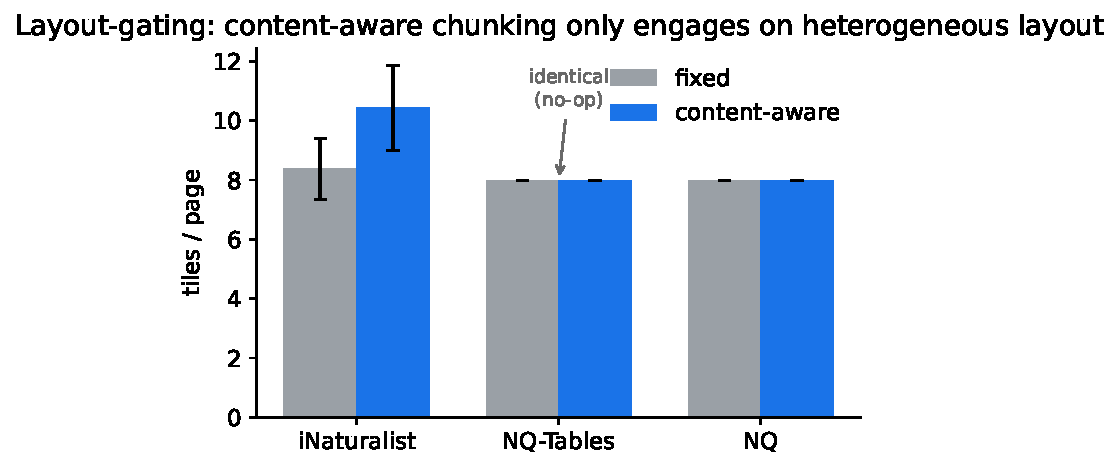
\includegraphics[width=0.74\linewidth]{fig1_layout_gating}
  \caption{\textbf{Layout-gating.} Content-aware chunking changes the tiling only on heterogeneous
  layout (iNaturalist); on the uniformly-formatted text corpora it is a no-op (identical tiles/page).}
  \label{fig:gating}
\end{figure}

\begin{table}[t]\centering
  \caption{Tiling, fixed vs.\ content-aware (CA), per corpus. CA is a byte-identical no-op on the uniform
  text corpora and engages only on iNaturalist.}
  \label{tab:layout}
  % AUTO-GENERATED by paper/gen_paper_numbers.py — DO NOT EDIT.
\begin{tabular}{lrrrr}
\toprule
Corpus & Tiles/pg (fixed$\to$CA) & Chunks (fixed$\to$CA) & Height std (fixed$\to$CA) & Engaged? \\
\midrule
iNaturalist & 8.38$\to$10.43 & 335$\to$417 & 82$\to$329 & yes \\
NQ-Tables & 8.00$\to$8.00 & 1680$\to$1680 & 2$\to$2 & \textbf{no-op} \\
NQ & 8.00$\to$8.00 & 1680$\to$1680 & 2$\to$2 & \textbf{no-op} \\
\bottomrule
\end{tabular}

\end{table}

\subsection{Retrieval}\label{sec:retrieval}
Table~\ref{tab:retrieval} reports article-level recall and nDCG per corpus per arm. On the text corpora,
content-aware chunking leaves retrieval essentially unchanged (it is the same tiling): NQ-Tables
recall@1 \NqtTxtRecallFixed/\NqtTxtRecallCa, NQ \NqTxtRecallFixed/\NqTxtRecallCa. On iNaturalist, the
effect of chunking on retrieval is \emph{modality-dependent}: image-query recall@1 rises
(\InatImgRecallFixed\ $\to$ \InatImgRecallCa), but text-query recall@1 \emph{falls}
(\InatTxtRecallFixed\ $\to$ \InatTxtRecallCa)---finer tiles fragment the gold page's text-match signal.
This sign difference foreshadows the QA result.

\begin{table}[t]\centering
  \caption{Retrieval (relevant modality per corpus). Content-aware chunking is neutral on the text
  corpora (identical tiles) and modality-split on iNaturalist.}
  \label{tab:retrieval}
  % AUTO-GENERATED by paper/gen_paper_numbers.py — DO NOT EDIT.
\begin{tabular}{llccc}
\toprule
Corpus (modality) & Chunker & R@1 & R@5 & nDCG@10 \\
\midrule
iNaturalist (image) & fixed & 0.88 & 1.00 & 0.51 \\
 (image) & content-aware & 0.96 & 0.96 & 0.51 \\
\midrule
NQ-Tables (text) & fixed & 0.85 & 0.89 & 0.71 \\
 (text) & content-aware & 0.85 & 0.89 & 0.71 \\
\midrule
NQ (text) & fixed & 0.88 & 0.92 & 0.75 \\
 (text) & content-aware & 0.88 & 0.92 & 0.75 \\
\bottomrule
\end{tabular}

\end{table}

\subsection{QA ablation}\label{sec:qa}
Table~\ref{tab:qamain} gives the 4-cell QA accuracies for all three corpora. On iNaturalist (image
queries) content-aware chunking helps (\InatFixedFlatAcc\ $\to$ \InatCaFlatAcc\ at flat retrieval) and
hierarchical expansion compounds it (\InatCaHierAcc). On the two text corpora content-aware chunking is within noise of fixed
(it is the same tiling): NQ-Tables flat \NqtFixedFlatAcc/\NqtCaFlatAcc, NQ flat
\NqFixedFlatAcc/\NqCaFlatAcc. The headline number---content-aware $+$ hier-expand reaching
\InatCaHierAcc\ on iNaturalist---is significant by an exact paired McNemar test against the fixed-flat
baseline (Table~\ref{tab:mcnemar}, contrast \textsc{C3}: $\Delta=\McNemarDelta$, $p=\McNemarP$, all
\McNemarFavor\ of \McNemarDiscordant\ discordant pairs favoring the full method). We report this number
\emph{only alongside its qualification in \S\ref{sec:modflip}}: it does not survive a query-modality flip.

\begin{table}[t]\centering
  \caption{QA accuracy, 4-cell ablation per corpus. Content-aware chunking helps only on iNaturalist
  (image queries); on the text corpora it is within noise (identical tiling). \textbf{Bold} is the
  iNaturalist headline, qualified in \S\ref{sec:modflip}.}
  \label{tab:qamain}
  % AUTO-GENERATED by paper/gen_paper_numbers.py — DO NOT EDIT.
\begin{tabular}{llcc}
\toprule
Corpus (query) & Chunker & Flat & Hier-expand \\
\midrule
iNaturalist (image) & fixed & 0.44 & 0.40 \\
 & content-aware & 0.56 & \textbf{0.68} \\
\midrule
NQ-Tables (text) & fixed & 0.49 & 0.54 \\
 & content-aware & 0.49 & 0.52 \\
\midrule
NQ (text) & fixed & 0.64 & 0.59 \\
 & content-aware & 0.61 & 0.61 \\
\bottomrule
\end{tabular}

\end{table}

\begin{table}[t]\centering
  \caption{Exact paired McNemar tests on the iNaturalist image-query 4 cells ($n=\McNemarN$).
  $^\star$ denotes $p<0.05$. The significant best-vs-baseline gain (\textsc{C3}) is qualified by
  \S\ref{sec:modflip}.}
  \label{tab:mcnemar}
  % AUTO-GENERATED by paper/gen_paper_numbers.py — DO NOT EDIT.
\begin{tabular}{lllccc}
\toprule
ID & Contrast & Arms & $\Delta$acc & Discordant (b:c) & $p$ (exact) \\
\midrule
C1 & Chunking (flat) & fixed\_flat$\to$ca\_flat & +0.12 & 0:3 & 0.250 \\
C2 & Expansion (CA) & ca\_flat$\to$ca\_hier & +0.12 & 0:3 & 0.250 \\
C3 & Best vs.\ baseline & fixed\_flat$\to$ca\_hier & +0.24 & 0:6 & 0.031\,$^\star$ \\
C4 & Expansion (fixed) & fixed\_flat$\to$fixed\_hier & -0.04 & 1:0 & 1.000 \\
\bottomrule
\end{tabular}

\end{table}

\subsection{The modality flip (cleanest evidence)}\label{sec:modflip}
To isolate the content-aware benefit from everything it co-varies with, we hold the iNaturalist corpus
\emph{and the content-aware tiles fixed} and change only the query modality from image to text---reusing
the identical retrieved tiles' provenance. Table~\ref{tab:modflip} and Figure~\ref{fig:modflip} show the
result. Under image queries the content-aware effect is \CaImgFlatDelta\ (flat) and \CaImgHierDelta\
(hier-expand); under text queries on the same corpus and tiles it is \CaTxtFlatDelta\ and
\CaTxtHierDelta. \textbf{The advantage does not survive the modality flip}, which is the cleanest
evidence that the content-aware benefit is image-query-specific rather than a property of the chunking.

The mechanism is visible in how often the gold page reaches the reader. Under image queries retrieval is
saturated---the gold page is read \ImgFixedSawGold\%\ of the time for fixed and \ImgCaSawGold\%\ for
content-aware---so the retrieval penalty has no room to bite and the reading benefit surfaces. Under text
queries the gold page reaches the reader only \TxtFixedSawGold\%\ (fixed) vs.\ \TxtCaSawGold\%\
(content-aware): content-aware's finer tiles actively \emph{lower} gold-page retrieval.

\paragraph{Caveat, stated where the claim is made.} iNaturalist questions are \emph{deictic}
(e.g.\ ``what is the range of \emph{this} bird''), naming the entity only in the query image, so text
queries retrieve weakly and the text arm is partly retrieval-floor-limited---this is \emph{not} a
perfectly clean modality A/B. Crucially, however, content-aware chunking made text-query retrieval
\emph{worse} (gold-page recall \TxtFixedSawGold\%\ $\to$ \TxtCaSawGold\%), not merely ``failed to help,''
so the directional conclusion---that the content-aware advantage is contingent on image-query
retrieval---holds.

\begin{figure}[t]\centering
  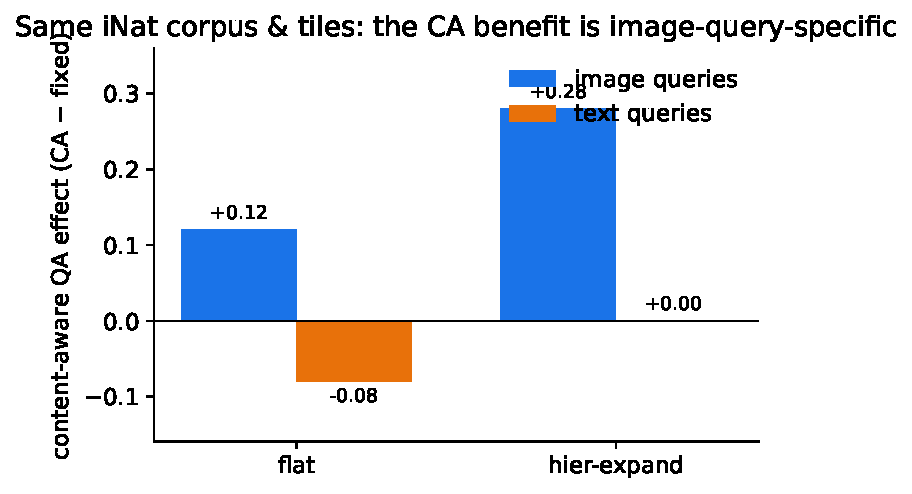
\includegraphics[width=0.72\linewidth]{fig2_modality_flip}
  \caption{\textbf{Modality flip (centerpiece).} Same iNaturalist corpus and tiles; only the query
  modality changes. The content-aware QA gain under image queries vanishes or reverses under text
  queries---it is image-query-specific.}
  \label{fig:modflip}
\end{figure}

\begin{table}[t]\centering
  \caption{Modality flip on iNaturalist (same corpus, same content-aware tiles). The content-aware effect
  (CA\,$\Delta$) is positive under image queries and non-positive under text queries.}
  \label{tab:modflip}
  % AUTO-GENERATED by paper/gen_paper_numbers.py — DO NOT EDIT.
\begin{tabular}{llccc}
\toprule
Modality & Retrieval & Fixed & Content-aware & CA $\Delta$ \\
\midrule
Image & flat & 0.44 & 0.56 & +0.12 \\
 & hier-expand & 0.40 & 0.68 & +0.28 \\
\midrule
Text & flat & 0.44 & 0.36 & -0.08 \\
 & hier-expand & 0.40 & 0.40 & +0.00 \\
\bottomrule
\end{tabular}

\end{table}

\subsection{The reader is the bottleneck}\label{sec:ceiling}
For each corpus's best content-aware configuration we classify every QA error as a \emph{reader ceiling}
miss (the gold page \emph{was} read but the answer was wrong) or a \emph{retrieval ceiling} miss (the
gold page was not in the reader's tiles). Figure~\ref{fig:ceiling} shows the split: iNaturalist
\InatReaderCeil:\InatRetrCeil, NQ-Tables \NqtReaderCeil:\NqtRetrCeil, NQ \NqReaderCeil:\NqRetrCeil---i.e.\
\ReaderCeilPctMin--\ReaderCeilPctMax\%\ of all errors are reading failures on \emph{correctly-retrieved}
content. In the hardest iNaturalist setting \emph{every} error is a reading failure on a retrieved gold
tile. Better chunking or deeper retrieval cannot fix a misread; the binding constraint is reader capacity.

\begin{figure}[t]\centering
  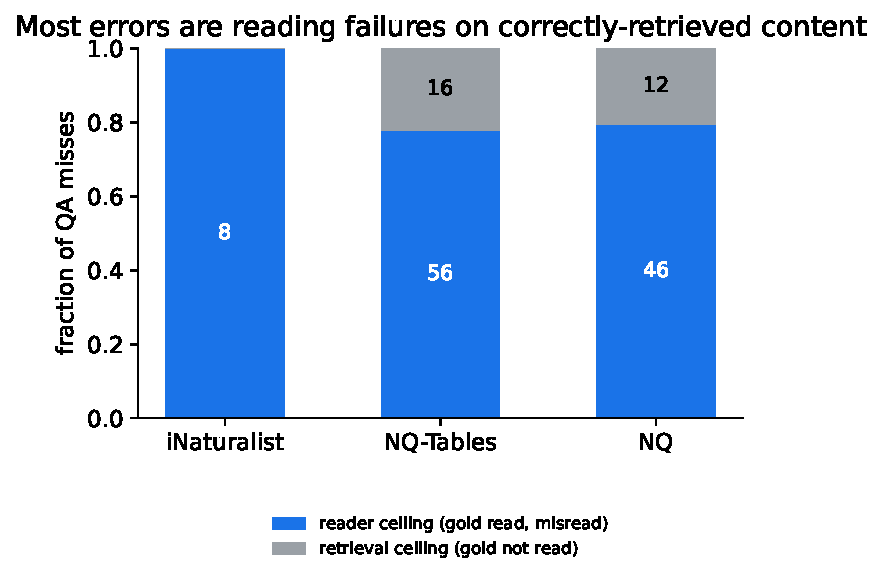
\includegraphics[width=0.7\linewidth]{fig3_reader_ceiling}
  \caption{\textbf{Reader-ceiling diagnostic.} Across corpora, most QA misses are reading failures on
  content the reader was correctly given (numbers are miss counts).}
  \label{fig:ceiling}
\end{figure}

\section{Discussion}\label{sec:discussion}
\paragraph{A reader--retriever tradeoff.} Content-aware chunking makes tiles smaller and content-aligned,
and these two consequences pull QA in opposite directions. Smaller, intact tiles are \emph{easier to
read}: the VLM sees a coherent region rather than a fragment spanning a boundary, so when the gold page
is in front of it, it answers more often. But smaller tiles also \emph{fragment the retrieval target}: a
page's content is spread across more, lower-mass embeddings, so a single query embedding matches the gold
page less reliably. Content-aware chunking is therefore not a strict improvement to ``the tiles''---it is
a \emph{reallocation} that helps the reader and hurts the retriever.

\paragraph{Query modality decides which effect dominates.} Under image queries on our encyclopedic
corpus, retrieval is already saturated (gold reaches the reader \ImgFixedSawGold--\ImgCaSawGold\%\ either
way), so the retrieval penalty cannot bite and the reading benefit surfaces as a QA gain (up to
\CaImgHierDelta). Under text queries on the \emph{same corpus and tiles}, retrieval is the binding
constraint; content-aware chunking lowers gold-page recall (\TxtFixedSawGold\%\ $\to$ \TxtCaSawGold\%) and
the QA advantage disappears or reverses. This within-corpus flip---holding document, layout, and chunk
difference fixed and changing only the query---is the cleanest evidence that the ``content-aware chunking
helps'' effect is contingent on the retrieval regime, not a property of the chunking itself.

\paragraph{Layout-gating.} Content-aware chunking can only express this tradeoff on documents whose
layout is heterogeneous enough that structure-aligned cuts differ from a fixed grid. On uniformly
formatted pages it produces identical tiles and is inert. An evaluation on uniform-layout corpora (much
of Wikipedia) will therefore report content-aware chunking as ``neutral''---but that is the absence of a
manipulation, not evidence about the method.

\paragraph{The reader is the bottleneck.} Across all three corpora,
\ReaderCeilPctMin--\ReaderCeilPctMax\%\ of errors occur on content the reader was correctly shown. For
practitioners of pixel RAG operating in this reader-bound regime, the highest-leverage investment is
reader capacity---a stronger VLM, better prompting, or answer verification---not chunking sophistication.

\paragraph{Practical guidance.} Do not adopt content-aware visual chunking expecting universal gains.
Expect it to (a) do nothing on uniform layouts, (b) help only when retrieval is not the binding
constraint (e.g.\ image-query or otherwise high-recall regimes), and (c) be dominated, in many real
pipelines, by the reader's reading capacity.

\paragraph{Future work.} Three directions follow directly from this study.
(i)~\emph{Reference-aware expansion}: our hierarchical retrieve-then-expand uses only
same-section siblings and $\pm1$ reading-order neighbors; following in-document
cross-references (figure/table callouts, ``see \S X'') to assemble the reader's context
would test whether reference-aware expansion recovers the retrieval mass that finer
content-aligned tiles fragment. (ii)~\emph{Breadth at scale}: extending the $2\times2$
ablation from three corpora to the full screenshot-RAG benchmark suite would establish
whether the reader--retriever tradeoff and layout-gating hold across document types and
larger $n$. (iii)~\emph{Tile-level retrieval metrics}: labeling answer-bearing tiles
would replace article-level recall/nDCG with a tile-level nDCG@$k$ that separates
retrieving the right \emph{page} from retrieving the right \emph{region}, sharpening the
diagnostic for where finer tiling helps or hurts.

\section{Limitations}\label{sec:limitations}
We state these as the boundary of valid claims, not as caveats to discount.
\begin{itemize}\setlength\itemsep{1pt}
  \item \textbf{Pilot scale.} The only corpus where the chunker engages, iNaturalist, has $n=\InatN$;
        the text corpora ($n=\NqtN$ each) are larger but are no-ops for the chunker.
  \item \textbf{The text arm is partly retrieval-floor-limited.} iNaturalist questions are deictic, so
        the modality flip (\S\ref{sec:modflip}) is not a perfectly clean A/B. Content-aware chunking made
        text retrieval \emph{worse}, not merely neutral, so the direction holds---but the magnitude under
        a cleaner text-query benchmark is unknown.
  \item \textbf{Single reader and judge.} All QA uses one reader (\texttt{\ReaderModel}) and one judge
        (\texttt{\JudgeModel}); the reader-ceiling result may shift with a stronger reader.
  \item \textbf{Closed mini-corpora.} We use gold-plus-distractor corpora, not full-scale open retrieval.
  \item \textbf{Co-varying corpora.} The three corpora differ on document type, query modality, and
        whether content-aware chunking engages; attribution across all three is partial. The cleanest
        causal claim is the within-corpus modality flip (\S\ref{sec:modflip}).
\end{itemize}

\section{Conclusion}\label{sec:conclusion}
Content-aware visual chunking is not a general improvement to screenshot RAG. It is a no-op on
uniform layouts; where it changes the tiling, it trades better reading against worse retrieval, so its
QA effect is image-query-specific (up to \CaImgHierDelta\ under image queries, \CaTxtFlatDelta/\CaTxtHierDelta\
under text queries on the same corpus and tiles). And across every setting we examine, the dominant
bottleneck is not chunking or retrieval but the reader: \ReaderCeilPctMin--\ReaderCeilPctMax\%\ of errors
are reading failures on correctly-retrieved content. The actionable takeaways are to expect content-aware
chunking to help only on heterogeneous layouts under high-recall retrieval, and to invest in reader
capacity where pixel RAG is reader-bound.

\begin{figure}[t]\centering
  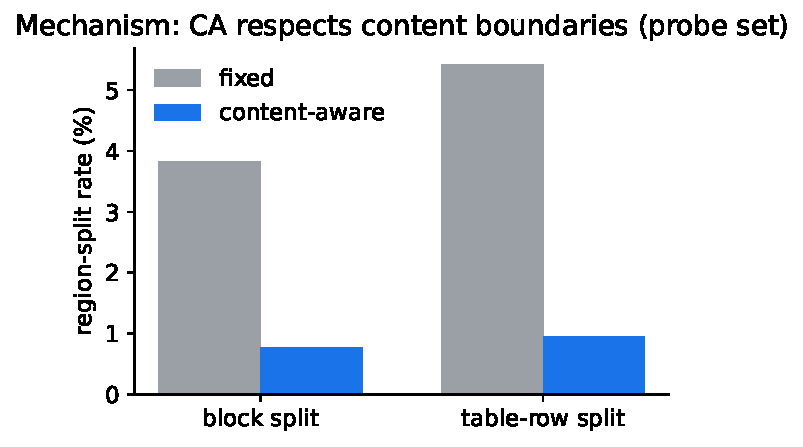
\includegraphics[width=0.6\linewidth]{fig4_boundary_violation}
  \caption{\textbf{Mechanism.} Region-split rate, fixed vs.\ content-aware, on the heterogeneous probe
  set: content-aware chunking respects block and table-row boundaries.}
  \label{fig:boundary}
\end{figure}

\begin{table}[t]\centering
  \caption{Boundary-violation rate on the probe set: content-aware chunking splits far fewer regions.}
  \label{tab:boundary}
  % AUTO-GENERATED by paper/gen_paper_numbers.py — DO NOT EDIT.
\begin{tabular}{lccc}
\toprule
Split type & Fixed & Content-aware & Reduction \\
\midrule
Block split & 3.82\% & 0.77\% & 5.0$\times$ \\
Table-row split & 5.42\% & 0.95\% & 5.7$\times$ \\
\bottomrule
\end{tabular}

\end{table}

\bibliographystyle{plainnat}
\bibliography{refs}

\end{document}
